\def\lecturenumber{02}
\documentclass[11pt,a4paper]{article}
\usepackage[T1]{fontenc}
\usepackage[utf8]{inputenc}
\usepackage{lmodern}
\usepackage[margin=19mm,top=21mm,bottom=21mm,headheight=15pt]{geometry}
\usepackage{amsmath,amssymb,booktabs,array,graphicx,microtype}
\usepackage[dvipsnames]{xcolor}
\usepackage{enumitem,fancyhdr,listings,tcolorbox}
\usepackage[colorlinks=true,linkcolor=MidnightBlue,urlcolor=MidnightBlue]{hyperref}
\definecolor{courseblue}{HTML}{164B69}
\definecolor{pale}{HTML}{F0F5F7}
\pagestyle{fancy}
\fancyhf{}
\fancyhead[L]{\small\sffamily\color{courseblue}VALIDATED COMPUTING}
\fancyhead[R]{\small\sffamily Lecture \lecturenumber}
\fancyfoot[L]{\footnotesize Expanded lecture notes \textbullet\ October 2026}
\fancyfoot[R]{\footnotesize\thepage\ / 6}
\renewcommand{\headrulewidth}{0.4pt}
\setlength{\parindent}{0pt}
\setlength{\parskip}{5.5pt plus 1pt}
\setlength{\emergencystretch}{1.5em}
\setlist[itemize]{leftmargin=1.5em,itemsep=3pt,topsep=3pt}
\setlist[enumerate]{leftmargin=1.7em,itemsep=5pt,topsep=4pt}
\lstset{language=Python,basicstyle=\small\ttfamily,keywordstyle=\color{courseblue}\bfseries,
 commentstyle=\color{OliveGreen},stringstyle=\color{BrickRed},showstringspaces=false,
 columns=fullflexible,keepspaces=true,frame=single,rulecolor=\color{black!18},
 backgroundcolor=\color{black!2},aboveskip=6pt,belowskip=6pt,breaklines=true,
 xleftmargin=5pt,xrightmargin=5pt,framesep=5pt}
\newcommand{\R}{\mathbb R}
\newcommand{\fl}{\operatorname{fl}}
\newcommand{\abs}[1]{\left|#1\right|}
\newcommand{\heading}[2]{\section*{\color{courseblue}#1}\vspace{-4pt}{\small\sffamily\color{black!65}#2}\par\vspace{3pt}}
\newcommand{\opening}[2]{{\Large\sffamily\bfseries\color{courseblue}Lecture \lecturenumber\quad #1\par}\vspace{5pt}{\small #2}\par}
\newtcolorbox{question}[1]{colback=pale,colframe=courseblue!55,boxrule=0.4pt,
 arc=1mm,left=7pt,right=7pt,top=4pt,bottom=4pt,title={#1},fonttitle=\bfseries\small,
 coltitle=courseblue,colbacktitle=pale}
\newcommand{\reading}[1]{{\footnotesize\textbf{Reading and notebook.} #1\par}}
\hypersetup{pdfauthor={Validated Computing course},pdfsubject={Expanded introductory lecture notes with questions and exercises}}

\hypersetup{pdftitle={Lecture 02: Floating-point numbers and rounding}}
\begin{document}
\opening{Floating-point numbers and rounding}{Prerequisites: Lecture 01, fractions, powers of two.\newline
Goal: predict what a floating-point operation can preserve, lose, or certify.}
\heading{1. Finite digits in a chosen base}{0--12 minutes: representation by hand before inspecting Python}
Writing a number with finitely many digits is a mathematical restriction. In base
two, a finite fractional expansion has the form
\[
 0.b_1b_2\cdots b_k=\sum_{j=1}^{k}b_j2^{-j}=\frac{m}{2^k},
 \qquad b_j\in\{0,1\}.
\]
Consequently a reduced rational $a/b$ has a finite binary expansion exactly when
$b$ is a power of two, ignoring the machine's exponent and precision limits.
If $a/b=m/2^k$ and $a,b$ are coprime, then $b$ divides $2^k$; conversely a
power-of-two denominator directly supplies a finite expansion. In base ten the
corresponding denominators may contain factors of both two and five.

Thus $3/8=0.011_2$ is exact in binary, while
$1/10=0.0001100110011\ldots_2$ repeats. The issue is not that a decimal literal
has ``too many digits'': one decimal digit can request a nonterminating binary
fraction. A finite machine format must select a nearby representable value.

\textbf{A toy format.} With $p=4$ significant binary digits, a positive normal
number is $(1.b_1b_2b_3)_2 2^e$. In $[1,2)$ its possibilities are
$1,1+1/8,1+2/8,\ldots,1+7/8$. Moving the exponent rescales this small grid.
The significand controls relative resolution; the exponent controls magnitude.
Do not confuse the two roles.

Python provides two useful descriptions of a stored float:
\begin{lstlisting}
x = 0.1
print(x.hex())               # 0x1.999999999999ap-4
numerator, denominator = x.as_integer_ratio()
print(numerator, denominator)
\end{lstlisting}
The hexadecimal string exposes the stored significand and a binary exponent.
The ratio is the exact rational value of that bit pattern. Neither description
claims that the stored value equals the intended rational $1/10$.
A short printed decimal is a convenient representation of the stored float,
not a transcript of every digit in its exact decimal expansion.

\begin{question}{Warm-up: justify each answer}
Which of $1/8$, $1/5$, $3/20$, and $13/16$ have finite binary expansions?
Write $13/16$ in binary. Would doubling the available precision make $1/5$
exactly representable? Separate representability from the quality of approximation.
\end{question}

\textbf{Generate the digits rather than memorizing them.} For $1/10$, start with
remainder $r=1$. At each step divide $2r$ by 10: its integer quotient is the next
binary digit, and its remainder becomes the new $r$. The remainders begin
$2,4,8,6,2,\ldots$; a repeated remainder restarts the same future digit sequence.
This finite-state calculation explains the repetition. Apply it to $1/8$ and
observe the remainder becoming zero. Terminating and repeating expansions are
consequences of integer arithmetic, not quirks of Python's display.

\newpage
\heading{2. Decode binary64 and derive its spacing}{12--30 minutes: fields, a worked decoding, and a number line}
The binary64 format has a sign bit $s$, an 11-bit stored exponent $E$, and a
52-bit fraction field interpreted as an integer $F$. For normal values,
\[
 x=(-1)^s2^{E-1023}\left(1+\frac{F}{2^{52}}\right),\qquad
 1\le E\le2046,\quad 0\le F<2^{52}.
\]
The leading one is implicit: there are $p=53$ significant binary digits even
though only 52 fraction bits are stored. The exponent bias is 1023.
\begin{center}\small
\begin{tabular}{@{}lcccc@{}}\toprule
Value & $s$ & $E$ & $F$ & Normalized form\\\midrule
$1$ & 0 & 1023 & 0 & $1.0_2\,2^0$\\
$1.5$ & 0 & 1023 & $2^{51}$ & $1.1_2\,2^0$\\
$-2.5$ & 1 & 1024 & $2^{50}$ & $-1.01_2\,2^1$\\\bottomrule
\end{tabular}
\end{center}
For $-2.5$, divide the magnitude by two to obtain $1.25=1.01_2$.
The unbiased exponent is one, and the fractional significand is $1/4$;
therefore $F/2^{52}=1/4$. This derives the fields rather than guessing their bits.

\textbf{Spacing theorem.} In a normal binade $[2^e,2^{e+1})$, consecutive values
are separated by $2^{e-(p-1)}$. Indeed, increasing $F$ by one changes the
significand by $2^{-(p-1)}$; multiplication by $2^e$ gives the stated step.
The spacing doubles at the next binade. Below an exact power of two, the
preceding normal binade has half the spacing of the one above.
\begin{center}
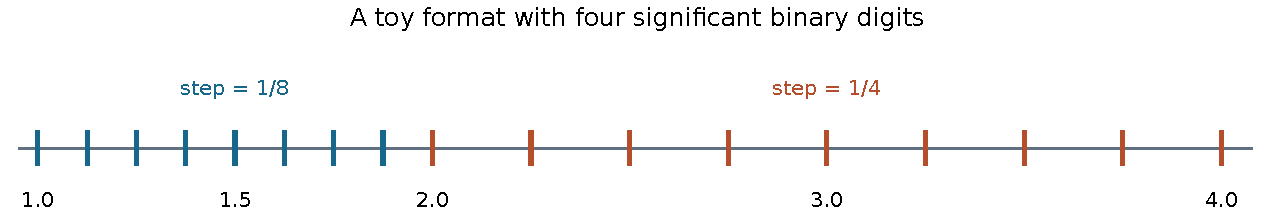
\includegraphics[width=0.93\linewidth]{figures/toy_spacing.pdf}
\end{center}
\begin{lstlisting}
import math
for x in [1.0, 2.0, 2.0**53]:
    below = math.nextafter(x, -math.inf)
    above = math.nextafter(x, math.inf)
    print(x, x - below, above - x)
\end{lstlisting}
At $1$, the lower and upper gaps are $2^{-53}$ and $2^{-52}$.
At $2^{53}$, they are $1$ and $2$. All integers from $0$ through $2^{53}$
are representable, but not all larger integers are. Precision is not a fixed
number of decimal places: absolute resolution changes with scale.
\begin{question}{Predict before running}
Why can $2^{53}-1$ be represented when $2^{53}+1$ cannot? What are the two
gaps at $2^{54}$? The smallest normal number is a special boundary; page 4 explains why.
\end{question}

The largest finite normal value is $(2-2^{-52})2^{1023}$: use the largest
normal exponent and set every fraction bit to one. This limit concerns
\emph{range}, whereas spacing concerns \emph{resolution}. Increasing the exponent
range alone would not let us distinguish $2^{53}$ from $2^{53}+1$ at 53-bit precision.

\newpage
\heading{3. Rounding modes and a one-operation bound}{30--48 minutes: prove the bound, then test midpoint cases}
Rounding to nearest selects a representable value closest to the exact result.
At an exact midpoint, \emph{ties to even} selects the neighbour whose last
significand bit is zero. It does not mean rounding every halfway value toward zero.
Directed rounding instead selects the neighbouring representable value below
or above the exact result. Those two modes will support interval endpoints later.

We use two distinct constants:
\[
 \varepsilon=2^{1-p}=2^{-52}\quad\hbox{(gap above 1)},\qquad
 u=2^{-p}=2^{-53}\quad\hbox{(unit roundoff)}.
\]
Some sources call either quantity ``machine epsilon'', so a symbol without a
definition is not enough. Our convention fixes $\varepsilon=2u$.

\textbf{Relative rounding bound.} For a nonzero exact value $z$ in the normal
range, assuming round-to-nearest and no overflow,
\[
 \fl(z)=z(1+\delta),\qquad |\delta|\le u.
\]
To prove this for $z>0$, take $2^e\le z<2^{e+1}$. The maximum distance to
a nearest neighbour is half a spacing, $2^{e-p}$. Dividing by
$z\ge2^e$ gives $|\fl(z)-z|/z\le2^{-p}$. Negative values follow by symmetry.
The normal-range assumption matters; it will fail in our next example.

For a correctly rounded basic operation, apply this statement to the exact result
of that operation on its \emph{stored operands}. Errors already present in the operands
have not disappeared. Nor does a sequence of a thousand operations acquire a
global relative-error bound of $u$ merely because each local rounding has such a bound.

\begin{lstlisting}
u = 2.0**-53
print(1.0 + u == 1.0)             # True: midpoint, even lower neighbour
print(1.0 + 3*u == 1.0 + 4*u)     # True: even upper neighbour
print(2.0**53 + 1.0 == 2.0**53)  # True: an exact increment is lost
\end{lstlisting}
In the last line both input operands are exact. The exact sum lies halfway
between $2^{53}$ and $2^{53}+2$; the first has the even low significand bit.
This is arithmetic rounding, not an inaccurate representation of the integer one.

\begin{question}{Small-group proof check}
Explain each inequality in the rounding-bound proof. Where were normal range,
nearest rounding, and exact operands used? If the exact result is zero, how would
you state an absolute-error claim without dividing by zero?
\end{question}
\textbf{Preview.} To enclose a compound expression, it is not enough to round its
final printed value outwards. Intermediate errors and dependencies also need
control. Interval arithmetic will organize those operations and their assumptions.

\textbf{A first accumulated-error calculation.} For stored inputs $a,b,c$, assume
the rounding model applies to both multiplications. Then
\[
 \fl(\fl(ab)c)=abc(1+\delta_1)(1+\delta_2),\qquad
 |\delta_1|,|\delta_2|\le u.
\]
The total relative error, when $abc\ne0$, is at most $2u+u^2$, not $u$.
This follows by expanding the product and applying the triangle inequality.
Even this tiny example needs a composed argument; cancellation in more general
expressions will make the analysis more delicate.

\newpage
\heading{4. The boundary of the model}{48--62 minutes: subnormals, exceptional values, and input provenance}
For normal binary64 numbers, the unbiased exponent ranges from $-1022$ to $1023$.
The smallest positive normal value is $2^{-1022}$. Exponent field $E=0$ uses
\emph{subnormal} values instead:
\[
 x=(-1)^s F\,2^{-1074},\qquad 1\le F<2^{52}.
\]
These have no implicit leading one. Their fixed spacing
$\alpha=2^{-1074}$ fills the gap towards zero. The gap just below the smallest
normal equals the gap just above it, unlike a boundary between two normal binades.
As magnitudes decrease through the subnormal region, relative precision deteriorates.

For example, the exact real $z=\alpha/2$ rounds to zero under ties to even.
Its absolute error is only $\alpha/2$, but its relative error is one.
A useful combined bound, excluding overflow, is
\[
 |\fl(z)-z|\le u|z|+\alpha/2.
\]
Normal results are covered by the relative estimate; in the tiny-value region,
nearest rounding has absolute error at most half the fixed spacing.
The extra absolute term accounts for gradual underflow.
\begin{lstlisting}
from fractions import Fraction
small = Fraction(1, 2**1075)
rounded = float(small)
assert rounded == 0.0
assert abs(Fraction.from_float(rounded) - small) / small == 1
\end{lstlisting}
\textbf{Special encodings.} $E=0,F=0$ represents signed zero. With $E=2047$,
$F=0$ represents an infinity and $F\ne0$ a NaN. Infinities and NaNs are not
ordinary real-number answers. In particular, \texttt{nan == nan} is false.
Python scalar division by zero raises an exception; NumPy arithmetic can instead
produce infinities or NaNs with warnings. A proof must specify the actual operation
semantics rather than assuming every programming interface behaves identically.

\textbf{More precision cannot repair the meaning of an input.}
\begin{lstlisting}
from decimal import Decimal, localcontext
with localcontext() as context:
    context.prec = 60
    intended = Decimal("0.1")
    inherited = Decimal(0.1)
    print(inherited - intended)
    print(Decimal(1) / Decimal(3))
\end{lstlisting}
The string denotes the exact decimal tenth; the float constructor preserves the
already-rounded binary input. The third still needs rounding at finite decimal
precision. Increasing the context changes later arithmetic, not earlier input history.

\newpage
\heading{5. A time-conversion error that grows with uptime}{62--77 minutes: exact model, operational bound, and historical context}
The GAO report on the 1991 Patriot failure describes precision loss when integer
clock ticks, counted in tenths of seconds, were converted to time. The tracking
error grew with operating duration; Appendix II reports about $0.3433$ seconds
at 100 hours. This was not a loop repeatedly adding Python's binary64 \texttt{0.1}.
The incident motivates a question: over what operating range is an error bound acceptable?
\href{https://www.gao.gov/assets/imtec-92-26.pdf}{[GAO IMTEC-92-26, pp. 5--6 and Appendix II]}

Use the following \emph{simplified fixed-point model}, not a reconstruction of the
historical software. Approximate $c=1/10$ seconds per tick by truncation to $q$
fractional binary bits:
\[
 \widehat c=\frac{\lfloor 2^q/10\rfloor}{2^q},\qquad
 0\le c-\widehat c<2^{-q}.
\]
For $N\ge0$ exact integer ticks, compare $t=Nc$ with $\widehat t=N\widehat c$.
In this model their difference is exact:
\[
 \Delta t=N(c-\widehat c),\qquad 0\le\Delta t<N2^{-q}.
\]
There is no random cancellation of the per-tick bias. Additional rounding of a
real implementation's multiplication would need another term; the model above
isolates the conversion-coefficient error.
\begin{lstlisting}
from fractions import Fraction
q = 23
scale = 2**q
tick = Fraction(1, 10)
stored_tick = Fraction(scale // 10, scale)
error_per_tick = tick - stored_tick
for hours in [1, 8, 24, 100]:
    ticks = hours * 3600 * 10
    error = ticks * error_per_tick
    print(hours, error, float(error))
\end{lstlisting}
Here $c-\widehat c=1/10485760$ seconds. At 100 hours,
$N=3600000$ and $\Delta t=5625/16384\approx0.343322754$ seconds.
Matching the scale of the historical table does not establish equivalence with
all details of the historical implementation.

\textbf{Design from a tolerance.} To guarantee a model error below $\tau$ over
$N_{\max}$ ticks, it suffices to choose $q$ with $N_{\max}2^{-q}\le\tau$.
Round-to-nearest gives a coefficient-error bound of $2^{-q-1}$ instead.
If the true tick length is uncertain by at most $\eta$, add $N\eta$ to the
conversion bound. More coefficient bits do not remove physical clock uncertainty.
\begin{question}{Design exercise}
For 100 hours and $\tau=0.01$ seconds, find a sufficient $q$ using the general
truncation bound. Explain why an uptime limit belongs in the specification.
\end{question}

\newpage
\heading{6. Exercises and a rounding audit}{77--90 minutes: compare explanations; complete remaining calculations after class}
Use exact fractions for reference values whenever possible. State whether you are
discussing an input conversion, one arithmetic operation, or an entire algorithm.
\begin{enumerate}
\item \textbf{Decode a value.} Write $6.5$ in normalized binary form and give its
binary64 fields $s,E,F$. Find its neighbours' spacing. Repeat the spacing question
at $8$ and explain why the lower and upper gaps now differ.
\item \textbf{Tie-breaking.} Work in a toy binary format with $p=4$ and sufficient
exponent range. Round $1+1/16$, $1+3/16$, and $2+1/8$ to nearest, ties to even.
For each, name both neighbours and identify the even significand. Do not use a
binary64 calculation as a substitute for this toy-format calculation.
\item \textbf{A lost integer.} Predict the binary64 results of adding $1$, $2$,
and $3$ to $2^{54}$. Explain why subtracting $2^{54}$ afterwards cannot recover
the discarded information. Which additions involve a midpoint tie?
\item \textbf{An input audit.} Compare \texttt{Fraction("0.1")} with
\texttt{Fraction(0.1)}.\\ Then compare \texttt{Decimal("0.1")} with
\texttt{Decimal(0.1)}.
Which preserve the intended decimal tenth, and which preserve the stored float?
Would setting a decimal precision of 100 change these input meanings?
\item \textbf{Bound the time error.} Derive the page-5 bound directly from the
floor inequality. For $q=23$, give a sufficient maximum integer tick count that
keeps the general bound at most $0.1$ seconds. Compare it with what is permitted
using the exact coefficient error. Explain why agreement at one uptime is not
a proof about all possible runtimes or implementations.
\end{enumerate}
\textbf{Selected checks.}
Exercise 1: $6.5=1.101_2\,2^2$, so $s=0$, $E=1025$, and $F=5\cdot2^{49}$;
its spacing is $2^{-50}$. At $8$, the lower gap is $2^{-50}$ and the upper gap
$2^{-49}$. Exercise 2 gives $1$, $1.25$, and $2$. Exercise 3 gives
$2^{54}$, $2^{54}$, and $2^{54}+4$. For the page-5 design exercise, $q=29$
is sufficient. Check each answer by explaining its rounding or bound, not just
by matching the number.

\begin{question}{Exit ticket}
State the meanings of $\varepsilon$ and $u$. Give one hypothesis needed for
$\fl(z)=z(1+\delta)$ with $|\delta|\le u$, and a concrete counterexample when
that hypothesis is removed. Which mistake would persist even at 200-digit precision?
\end{question}
\reading{Companion: \texttt{notebooks/02\_floating\_point.ipynb}; Lab 02: inspect the machine.
Tucker (2011), \S\S1.2--1.5. See the
\href{https://docs.python.org/3/tutorial/floatingpoint.html}{Python floating-point tutorial}
and \href{https://docs.python.org/3/library/decimal.html}{Decimal documentation}
for Python interfaces. Historical source: GAO IMTEC-92-26 (1992), linked on page 5.}
\end{document}
